% v2-acmtog-sample.tex, dated March 7 2012
% This is a sample file for ACM Transactions on Graphics
%
% Compilation using 'acmtog.cls' - version 1.2 (March 2012), Aptara Inc.
% (c) 2010 Association for Computing Machinery (ACM)
%
% Questions/Suggestions/Feedback should be addressed to => "acmtexsupport@aptaracorp.com".
% Users can also go through the FAQs available on the journal's submission webpage.
%
% Steps to compile: latex, bibtex, latex latex
%
% For tracking purposes => this is v1.2 - March 2012
\documentclass{acmtog} % V1.2

%\acmVolume{VV}
%\acmNumber{N}
%\acmYear{YYYY}
%\acmMonth{Month}
%\acmArticleNum{XXX}
%\acmdoi{10.1145/XXXXXXX.YYYYYYY}

\acmVolume{28}
\acmNumber{4}
\acmYear{2019}
\acmMonth{January}
\acmArticleNum{106}
\acmdoi{10.1145/1559755.1559763}

\begin{document}

\markboth{V. F. Pamplona et al.}{Photorealistic Models for Pupil Light Reflex and Iridal Pattern Deformation}

\title{A New GA Trials for NP problems} % title

\author{SUO QIU {\upshape and} PENGBO NIE
\affil{Shanghai Jiao Tong University}
% NOTE! Affiliations placed here should be for the institution where the
%       BULK of the research was done. If the author has gone to a new
%       institution, before publication, the (above) affiliation should NOT be changed.
%       The authors 'current' address may be given in the "Author's addresses:" block (below).
%       So for example, Mr. Fogarty, the bulk of the research was done at UIUC, and he is
%       currently affiliated with NASA.
}





\maketitle


\section{Introduction}

\begin{figure*}[t]

\centerline{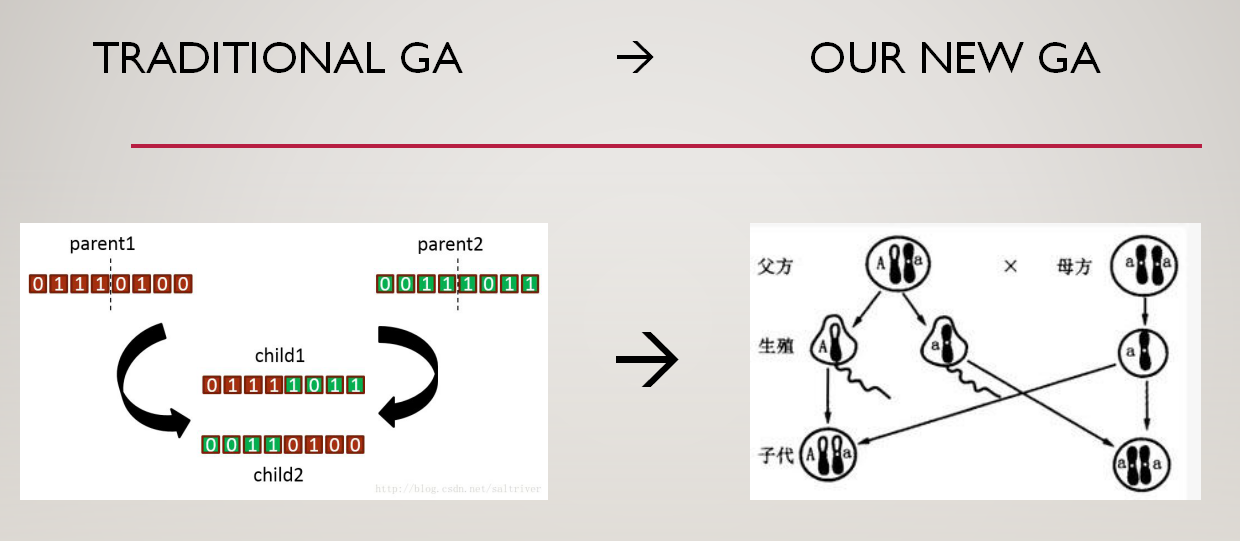
\includegraphics[width=15cm]{1}}


\caption{Comparison of the tradition GA generation idea with our new GA formation.

\ \ \ \ \ \ \ \ \ \ \ \ \ \ The traditional GA: one gene chain, one cross and one combination.

\ \ \ \ \ \ \ \ \ \ \ \ \ \ Our new GA: consists of two chains considering both the dominant genes and the recessive genes to increase the diversity of offspring.}

  \label{fig:comparison}
\end{figure*}

\ \ \ We start with the idea of a new GA algorithm by changing the traditional Genetic Algorithm's binary coding way into a method considering both dominant genes as well as recessive genes to increase the diversity of their every offspring generation.

Compared with old-GA methods, the new coding way is more alike the natural genetic hybrid way and distinguishes the Explicit-implicit relationship between genes and their corresponding performance, which may lead to a  better results.
    
In this article, we present this new GA method to all of you. There're always many attempts to improve the GA algorithm about cross method, mutation method, and combining other algorithms...but very few in this way: change the coding way of GA. We will illustrate it part by part to make it more concrete and understandatble. We'll first refer to the nowadays background of GA and the related works done in improving, which is our first two parts. Then there actually still are drawbacks that all these former works didn't solve. Combining our biology knowledge and the aim to deal with the drawbacks we show our idea motivation next and the problem formulation in part 5. After finishing this we step to a closer look at our new GA method.  Comparison of the tradition GA generation idea with our new GA form is vividly shows in Figure.1 and Figure.2 is the comparison  between  the  old  GA  technological  process  and  our
new GA’s process. They're both contained in the part of our new GA process method presentation. And in the Experiment part, we will show in a serial order our first trial in n-queens, our main trial in TSP and our extension trial on 3-SAT with all four steps:
1. How to make gene table. 
2. Gene chains to performance. 
3. How to in-cross. 
4. How to choose mutation. 
illustrated respectively. With description as a reminder of the problem and our own result. Figure.3,4,5,6 are our applied in-cross method in TSP and they'll help in understanding. In the final of the report we make a conclusion of our whole trial. All the new GA's code is implemented by ourselves. (There's no need to list the former references in the stage of idea formulation, that's too many.)


\section{Background}
\label{sec:background}
\ \ \ Nowadays, Genetic Algorithm is widely used in a variety of questions especially in NP-hard problems, among which TSP is the most familiar problem to us.

Genetic Algorithm can now quite rapidly limit the population to a convergence value. But in the post several generations, because of the chromosome of different individuals in this population being so close that we can hardly get a some kind of “new” chromosome in the future generations, thus the result we get cannot jump out of the local maximum for sure. But if we merely increase the mutation frequency, which will cause an oscillation effect

\section{Related works}
\label{sec:related_works}

\ \ \ \ The Drawbacks of existing algorithm: (Aiming to solve TSP problem)

1. An improvement of Genetic Algorithm by judging by the \emph{abort algebra} (2013): raise the convergence performance but also easily stucking in local optimum.

2. \emph{Greed Cross-3PM} Based on Simulated Annealing Genetic Algorithms (2010): the optimizing result graph shows the inter-related phenomenon.

3. \emph{ISAGA} (improved genetic simulated annealing algorithm: using self-adapting Metropolis theory to amend offspring) (2016): very limited optimizing results.

As the current algorithms mostly focus on properly lengthening the lifespan of heritance of some “bad genes” to maintain the diversity of samples, we are looking forward to proposing a new genetic algorithm which has good convergence and is not easy to fall into local optimum thus avoiding the current drawbacks to solve the unsolved problems like TSP. 


\section{idea Motivation}
\label{sub:idea_motivation}

\ \ \  Inspired by the dominating status that diplont in natural world and the brilliant heredity and variation of Sexual reproduction.

Genes exist in the form of gene pairs. Characters are determined by the dominant and recessive relationship between a pair of genes. Gene pairs exist on the basis of chromosome pairs. Gene diversity can be achieved through the presence of recessive genes (traditionally we only consider the dominant genes).


\section{Problem Formulation}
\label{sec:problem_formulation}
\ \ \ \ \emph{Brief Algorithm}: We change the traditional Genetic Algorithm's binary coding way into a method considering both dominant genes as well as recessive genes to increase the divercity of their every offspring generation.

\emph{Goal}: Solving the problems of the original way: too early convergence and thus easily to stuck in local optimum.

\emph{Problems related}: TSP and so on (performed better in optimization)


\section{new GA process methods implementation}
\label{sec:process_methods}
%
\ \ \ \ Here comes to the achieving part. For an old GA, we need four procedures to create a new generation: first calculate fitness, then do selections mostly by means of Roulette to choose the target sample parents, cross them, with mutation afterwards.

As for ours, decide the outward manifestation is the first step that needs to be done, which is based on the gene table we built. It’s a table which shows the Explicit-implicit relationship between genes and thus we can tell the external manifestation or the single one performance character from two genes accordingly. 

Then the fitness calculation, selection and mutation remains similarly. 

The hybrid section, expanded from the cross section, our first thought is for each gene pair, we choose one gene to be inherited. Shortly afterwards it is denied, for it’s too complicated and will create N triple level comparison numbers for each chain. We later use a method called in-cross, which means the two chains in one parent will first cross internal and then apply chain recombination which is each parent giving one chain and later combined together to form a new child, which is exactly corresponding to the homologan chromosome crossing over with meiosis in the nature.

\begin{figure}[ht]
\centering
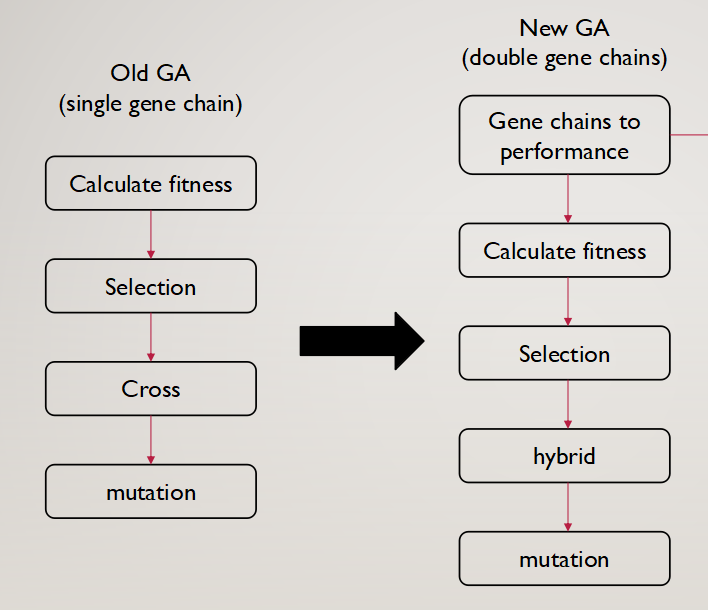
\includegraphics[scale=0.5]{2}
\caption{Comparison between the old GA technological process and our new GA's process }
\label{fig:label}
\end{figure}


\section{experiment}
\label{sec:experiment}
%
\ \ \ \ Now we implant our thoughts into experiments. We start from N-queens problems and then mainly dig its potential in TSP problems and the last extension to 3-SAT problems. All using our new GA idea but with each different gene table, in-cross methods, mutation methods according to concrete problems.
 
\subsection{First try ---- N Queens Problem}
\label{subsec:nqueens}
Our first try is N-queens problem, as an feasibility analysis of our idea, to prove its superiority. 

\subsubsection{N Queens Description}
\label{subsubsec:nqueensdescription}
\qquad

The n-queens puzzle is the problem of placing n queens on an n×n chessboard such that no two queens attack each other.

In n-queens the old GA representation is a single chain containing n numbers range from 1 to n to show the position of the queen in i'th column and j'th row. We maintain this representation method only extend it into two chains with following operations to make it work.



\subsubsection{N Queens gene table}
\label{subsubsec:nqueensgenetable}
\qquad

Randomly generate two positions for queen (one dominance and one recessive) in every column as our initial genes. And we randomly build a fixed table to represent the priority of explicit-implicit of the genes.

\subsubsection{N Queens gene to performance}
\label{subsubsec:nqueensperformance}
\qquad

Just need to refer to the gene table to decide which gene is in dominance place and be the outer performance.

\subsubsection{N Queens in-cross}
\label{subsubsec:nqueenscross}
\qquad

The two chains in one parent will first cross internal and then apply chain recombination which is each parent giving one chain and later combined together to form a new child.

The internal cross is same as the ordinary cross: head of the first chain attached to the tail of the second chain.

\subsubsection{N Queens mutation}
\label{subsubsec:nqueensmutation}
\qquad

Same as old mutation: A gene randomly transformed to a new gene.

\subsubsection{N Queens running results}
\label{subsubsec:nqueensresults}
\qquad

The results we got is quite promising, as the 8 queens problem is optimized. It won't stop until the optimal results achieved. It always takes tradition GA nearly 6000 steps to achieve the final goal but we only need 2000 steps. The reason we think about is the traditional GA with less diversity is hard to jump out of local optimum while as for our new approach, that'll be much easier. 


\subsection{Main try ---- TSP Problem}
\label{subsec:tsp}
The success in N-queens problems gives us power and faith to apply the new GA to TSP problem.

\subsubsection{TSP Description}
\label{subsubsec:tspdescription}
\qquad

The travelling salesman problem (TSP) asks the following question:"Given a list of cities and the distances between each pair of cities, what is the shortest possible route that visits each city and returns to the origin city?" It is an NP-hard problem in combinatorial optimization, important in operations research and theoretical computer science. 

In TSP, first we set a serial number of all the cities, supposing the number of which is n. The old GA representation is a single chain containing n numbers range from 1 to n but only once. The serial position in the chain of the city number is the serial visiting sequence of the visitor. We maintain this representation method only extend it into two chains with following operations to make it work.

\subsubsection{TSP gene table}
\label{subsubsec:tspgenetable}
\qquad

Our first think is: the later a certain gene appears, the lower priority they have.

But as the sample number is quite large so maybe almost all possibilities will exist in the initial generation. We tried three ways instead.

1. Sequential gene table: the priority of the cities equates the serial assigned number of the city. (for instance the city numbered 0 has the highest priority and so on)

2. Random gene table: the priority corresponding to each city is randomized.

Both of above two are fixed gene table and once established, it will not change.

3. Changeable gene table: once a mutation completed, change the priority of the changed gene.

The running results of former two fixed gene table is better than the changeable one as we tried. The changeable gene table will lead to unbearable low convergence rate so we then abandoned it.


\subsubsection{TSP gene to performance}
\label{subsubsec:tspperformance}
\qquad

The transformation from genes to character performance, which we do based on gene table. And of course in TSP there’ll be conflicts if more than once the same city appears on the chain. Towards those conflict points, we may select the unchosen cities in random or sequential and fill them in. That's called \emph{Random search} and \emph{Sequential search}.

We later improve it by selecting the index or priority nearby points closest to the conflict ones. We call them \emph{Index nearby search} and \emph{Priority nearby search}.

At last we think of the allele: choose dominant gene first, if conflicts, choose the recessive one, if conflicts again, we choose from above four methods to find one. In this way, not only the number of conflicts to deal with is much smaller, but also the association is more tight between genes and its corresponding character performance.


\subsubsection{TSP in-cross}
\label{subsubsec:tspcross}
\qquad

The in-cross principle is unbreakable. And on basis of that we make improvements on the method of internal cross as well as dealing with conflicts (the most crucial problem in TSP).

\qquad

{\bfseries 1. Simple Cross:}

We first choose a simple cross method: exchange the tail part of the chain, count the conflicts in tails of both chains and randomly allocate them on the other chain.

\begin{figure}[ht]
\centering
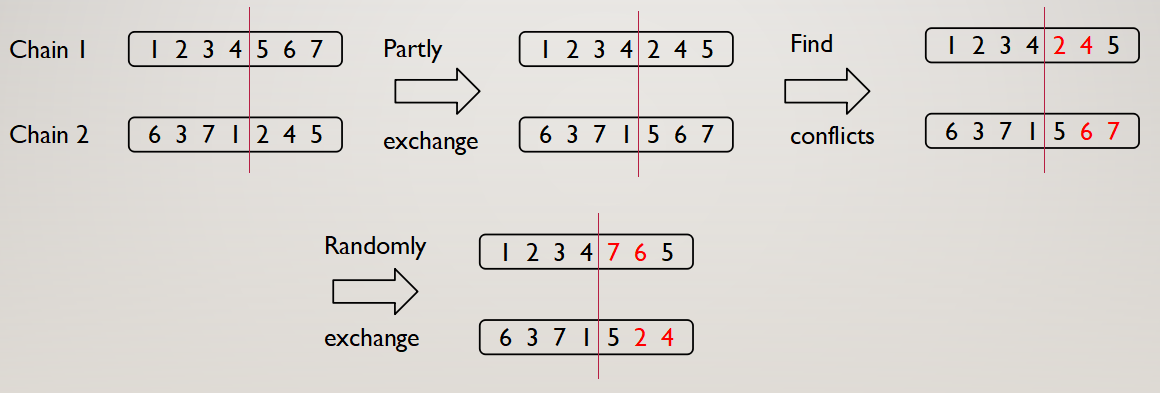
\includegraphics[scale=0.35]{3}
\caption{Simple Cross}
\label{fig:label}
\end{figure}

{\bfseries 2. Partly Swap:}

We next improve it into partly swap: exchange the mid part. We deal with the conflicts in the way of replacements. Let’s take the upper chain for example: 1,2 are conflicts, change 1,2 in the head of the upper chain with middle-responding 4,5 in the lower chain. After former operation, 4 is now a new conflict, exchange it with middle-responding 6. Done! No conflicts now. Same operation will be applied to chain 2 to make it right. 

\begin{figure}[ht]
\centering
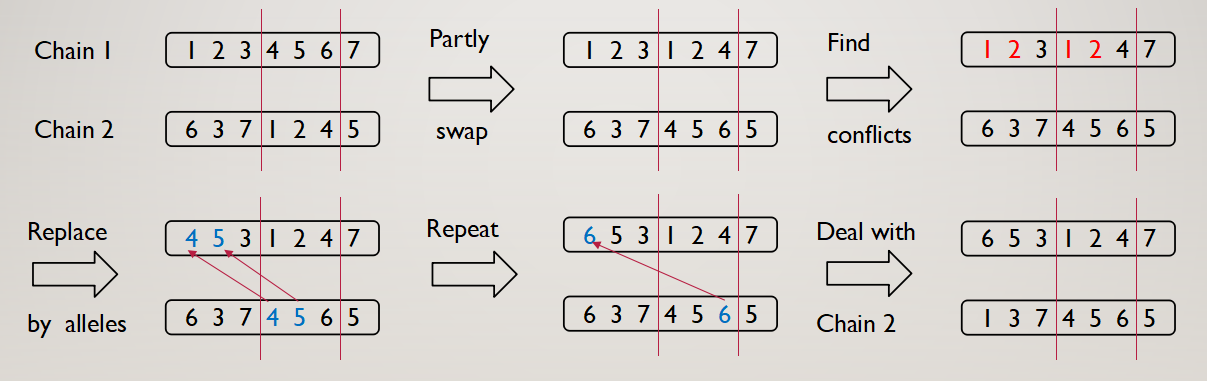
\includegraphics[scale=0.35]{4}
\caption{Partly Swap}
\label{fig:label}
\end{figure}

{\bfseries 3. Fetch and Rearrangement:}

Fetch a part, rearrange it with sequential not changed is another way we tried. Fetch a random part in the middle of the lower chain, arrange it exactly at the head of the upper chain, followed by not conflicted genes in the upper chain remaining sequential(if 3 is before 4 in the old chain, then it remains before in the new chain generated). Same operation applied to the second chain, or we can just rearranged the fetched part and put it ahead. 

\begin{figure}[ht]
\centering
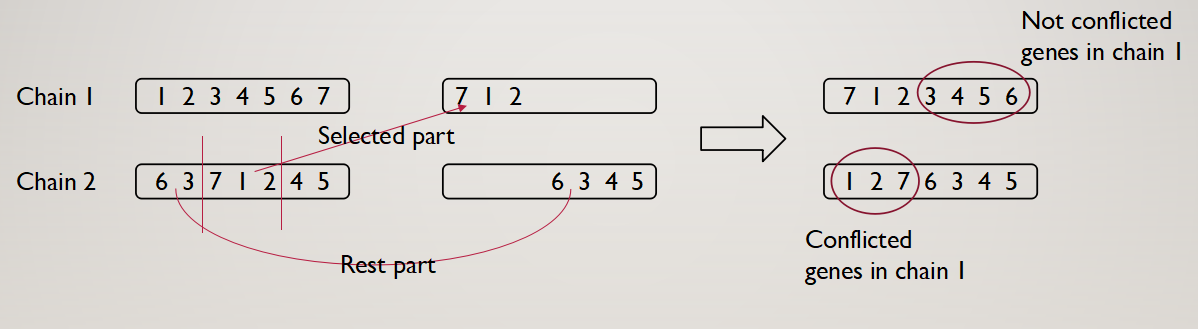
\includegraphics[scale=0.35]{5}
\caption{Fetch and Rearrangement}
\label{fig:label}
\end{figure}

{\bfseries 4. Merge:}

The last cross method we use is somewhat interesting. We call it merge, illustrated by following example shown in the picture: First check the first number of chain1, then the first number of chain2, then the second number of chain1, the second number of chain2, and the third number of chain1 ... if no conflict, put it in chain1, otherwise, locate it in chain2. This operation will bring us two generated chains with no conflicts.

\begin{figure}[ht]
\centering
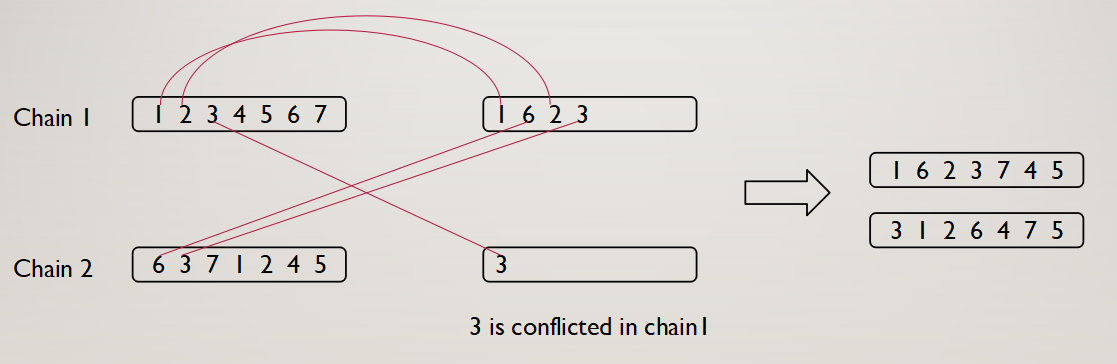
\includegraphics[scale=0.35]{6}
\caption{Merge}
\label{fig:label}
\end{figure}

All four methods used, the \emph{Fetch and Rearrangement} shows the current best results.

\subsubsection{TSP mutation}
\label{subsubsec:tspmutation}
\qquad

Traditional mutation method in TSP is just exchanging two genes' position.

In order to make an improvement for faster convergence: we mutate three times
In every mutation, if the new genes change the performance to a worse case, return to the origin gene chain. And if it is the third time mutation, no return.


\subsubsection{TSP running results}
\label{subsubsec:tspresults}
\qquad

The results of our new GA is currently not better than the traditional GA in TSP. Maybe we should consider it respectively in convergence rate (Running Faster) and better results (Path Optimization) afterwards.

\subsection{Extension ---- 3-SAT Problem}
\label{subsec:3sat}
The results didn't meet up with our expectations in TSP problem. So we tried another problem: 3-SAT, also a NP-Complete problem.

\subsubsection{3-SAT Description}
\label{subsubsec:3satdescription}
\qquad

SAT is the problem of determining if there exists an interpretation that satisfies a given Boolean formula. In other words, it asks whether the variables of a given Boolean formula can be consistently replaced by the values TRUE or FALSE in such a way that the formula evaluates to TRUE. If this is the case, the formula is called satisfiable. On the other hand, if no such assignment exists, the function expressed by the formula is FALSE for all possible variable assignments and the formula is unsatisfiable. 3-SAT is determining the satisfiability of a formula in conjunctive normal form where each clause is limited to at most three literals. It's NP-complete also. 

In 3-SAT, every variable takes the value 0 or 1, respectively. GA will form a string of chain whose length is n each representing a certain variable and with value 0 or 1. We maintain this representation method only extend it into two chains with following operations to make it work.

\subsubsection{3-SAT gene table}
\label{subsubsec:3satgenetable}
\qquad

Based on the experiences we get from TSP. We choose the fixed gene table. And for each variable whether the priority is 0 or 1 is random,

\subsubsection{3-SAT gene to performance}
\label{subsubsec:3satperformance}
\qquad

Just need to refer to the gene table to decide which gene is in dominance place and be the outer performance. No conflict to deal with.

\subsubsection{3-SAT in-cross}
\label{subsubsec:3satcross}
\qquad

Stick to the in-cross principle. And as for the internal cross we choose the ordinary simple cross: head of the first chain attached to the tail of the second chain.

\subsubsection{3-SAT mutation}
\label{subsubsec:3satmutation}
\qquad

Each variable has a certain number of chance of mutation, for instance 0.05, to change from 0 to 1 or 1 to 0 in the generating process.

\subsubsection{3-SAT running results}
\label{subsubsec:3satresults}
\qquad

For an optimized sample data with 30 variables and 129 clauses. The old GA normally need average 300 steps to achieve the final optimal result.`But our new GA need average 700 plus steps to achieve that.

That's frustrating. And the clue is extremely confused for our 3-SAT modeling is quite similar to n-queens but the result superiority is exactly the opposite.


\section{Conclusion}
\label{sec:conclusion}
%
\ \ \ \ The topic of our project is New Genetic Algorithm for NP problems. But after the success trial in n-queens problem. Our later mainly application on TSP's result turns out not good enough. We extend it to 3-SAT but the performance is surprisingly worse with similar model and process. So this new trial didn't meet up with its initial goal, which is disappointing. 

However, from the idea generation to problem formulation to experiment. That's a long road with our enthusiasm and effort and thanks to all teacher's and fellows' help. It is a real worthwhile and meaningful trial and our first-time systematic research onto a brand-new idea of ourselves.

Only gratitude.


\end{document}
% End of v2-acmtog-sample.tex (March 2012) - Gerry Murray, ACM
